\originalchapter{研究生作业五：介质力与因果响应}
题面据8.311作业5全部6题, 解答为AI独立推导. 官方手写解答采用负应力$\mathcal T=-T$, 且明确$\vct F=-\oint\mathcal T\cdot\nn\dd a$; 原题同一负应力写正面积积分属于符号误印. 本章统一用第8章正应力和外向法线.
\originalsection{介质应力及边界力}
\begin{exercise}
原题1. (a) 对线性介质$\vct D=\varepsilon\ee$、$\bb=\mu\vct H$导出应力及合力积分; (b) 真空–介质平面外电场分别法向和切向, 求单位面积力并与逐电荷受力解释比较.
\end{exercise}
\begin{solution}
(a) 静态、各向同性时$T_{ij}=E_iD_j+H_iB_j-(\ee\cdot\vct D+\vct H\cdot\bb)\delta_{ij}/2$. 用$\nabla\times\ee=0$、$\nabla\times\vct H=\jj_f$展开散度, 得
$\partial_jT_{ij}=\rho_fE_i+(\jj_f\times\bb)_i-E^2\partial_i\varepsilon/2-H^2\partial_i\mu/2$. 均匀介质内部后两项消失, 非均匀介质的材料力须保留. 动态还需动量时间变化, 不能把静态面积积分直接用于加速场而漏掉它. 该宏观应力采用忽略电致伸缩的材料模型; 真空应力给微观总Lorentz力, 不同介质动量划分还含机械部分.

(b) 法线$\nn$由介质指向真空, 取无自由面荷. 法向外场$E$时内场$E/\varepsilon_r$, 应力差$\vct f_s=\eps E^2(1-1/\varepsilon_r)\nn/2$. 切向两侧场同为$E$, 差为$\eps(\varepsilon_r-1)E^2\nn/2$. 两式由法向分量$T_{nn}$逐侧相减得到. 用虚功可核: 静电能变分含$-E^2\delta\varepsilon/2$, 移动介质面时积分介电率过渡, 法向保持$D_n$连续, 切向保持$E_t$连续, 便得到这两个牵引.

逐电荷的$\sum q_i\ee_{\rm ext}$须去除自身场并计入介质内部应力. 若只对理想零厚束缚电荷面用$\sigma_b\ee_{\rm av}$, 法向得到$\eps E^2(1-1/\varepsilon_r^2)\nn/2$, 与上述宏观材料牵引不同; 切向更没有净表面电荷可代表全部偶极作用. 差异说明不能用一层净面荷替代极化介质的完整机械模型. 官方解也以虚功处理介电率梯度并明确忽略电致伸缩项; 本书不把两种受力定义混同.
\end{solution}
\originalsection{固定电压和固定电流的吸入}
\begin{exercise}
原题2. (a) $L\times L$平板、间隔$d$, 电池固定电压$V$, 厚度近$d$的介质插入一半, 求吸入力; (b) 长$L$、半径$r$、总$N$匝螺线管恒流$I$, 同半径磁介质柱插入一半, 求力.
\end{exercise}
\begin{solution}
以插入长度$x$增大为正, $C(x)=\eps L[(L-x)+\varepsilon_rx]/d$. 固定$V$须计电源功, 合势$-CV^2/2$给$F_x=\eps(\varepsilon_r-1)LV^2/(2d)$. 恒流磁情形相同逻辑用磁共能$I^2\mathcal L/2$, 匝密度$n_t=N/L$, $\mathcal L(x)=n_t^2\pi r^2[\mu_0(L-x)+\mu x]$, 所以$F_x=I^2n_t^2\pi r^2(\mu-\mu_0)/2$. 能量增加由电流源补给, 不能只取固定$I$场能的负导数. 忽略边缘场且介质线性无滞后; 原卷磁性材料的$\mu$是磁导率.
\end{solution}
\originalsection{镜面、介质表面和光镊}
\begin{exercise}
原题3. (a) 线偏振峰值$E_0$正入射半透明镜, 求平均力; (b) 正入射折射率$n$介质表面求力; (c) 5$\mu$m光斑托住直径4.5$\mu$m、密度1.05g/cm$^3$、折射率1.59乳胶球, 估计空气和水中所需功率.
\end{exercise}
\begin{solution}
(a) 同一真空两侧的功率系数$R,T$, 入射$I_0=\eps cE_0^2/2$, 动量账给$p=I_0(1+R-T)/c$. 理想无吸收镜$T=1-R$时$p=2RI_0/c$, 吸收部分也有动量, 不可一律只算反射.

(b) 对上节宏观介质应力, 入射向$+z$, 真空侧$\langle T_{zz}\rangle=-I_0(1+R)/c$, 介质侧$-nTI_0/c$, 所以界面牵引沿$+z$为$p=I_0(1+R-nT)/c=2I_0(1-n)/[c(1+n)]$. 对$n>1$是朝真空的表面牵引; 不代表整个介质样品总受力逆光, 出射面与内部机械动量也需计入. 此处$T=4n/(1+n)^2$是功率透射系数, 不能误用振幅平方$t^2$.

(c) 题面未指定束形或波长, 无唯一数值. 球半径$a=2.25\mu$m, 体积$4\pi a^3/3$, 空气重力$4.92\times10^{-13}$N, 水中扣浮力后$2.34\times10^{-14}$N. 5$\mu$m光斑与球直径相当, 受光比例为一阶量. 采用粗估$F\simeq Q n_hP/c$, 梯度效率$Q$取介电对比$C=(n_s^2-n_h^2)/(n_s^2+2n_h^2)$的量级. 空气$n_h=1$, $C=0.337$, 给$P\sim0.44$ mW; 水$n_h=1.33$, $C=0.125$, 给$P\sim0.056$ mW. 若只取$Q=0.1$, 分别为1.5mW和0.053mW. 因束形与陷阱轴向梯度不同, 这些是约毫瓦和十分之一毫瓦的估计. 对光学波长球未必满足$a\ll\lambda$, 故不把静态Rayleigh极化率当该尺寸的精确散射解. 官方空气估计约1mW, 其水中支未给明确数值.
\end{solution}
\originalsection{导体内外功率与焦耳热}
\begin{exercise}
原题4. 正入射欧姆导体: (a) 求导体外平均能流及反射功率; (b) 求内能流散度并核焦耳热.
\end{exercise}
\begin{solution}
令$N=n+i\kappa=\sqrt{1+i\sigma/(\eps\omega)}$, $r=(1-N)/(1+N)$, $t=2/(1+N)$. 外部净输入$\langle S_z\rangle=I_0(1-|r|^2)$, 反射$|r|^2I_0$. 内部$\langle S_z(z)\rangle=\eps c n|tE_0|^2e^{-2\omega\kappa z/c}/2$. 用$2n\kappa=\sigma/(\eps\omega)$得$-\partial_z\langle S_z\rangle=\sigma|tE_0|^2e^{-2\omega\kappa z/c}/2=\langle\jj\cdot\ee\rangle$. 在表面输入连续, 全半空间吸收等于净输入. 官方(b)只有起式, 上述散度与积分是独立补算.
\end{solution}
\originalsection{记忆核、导数展开与极化激元}
\begin{exercise}
原题5. $\varepsilon_r(\omega)=1+\omega_p^2/(\omega_0^2-\omega^2-i\gamma\omega)$. (a) 把时间卷积写为导数级数至少至二阶; (b) 求小耗散色散和群速, 示意作图.
\end{exercise}
\begin{solution}
写$\vct D=\eps[\ee+\int G(\tau)\ee(t-\tau)\dd\tau]$, $G=\Theta(\tau)\omega_p^2e^{-\gamma\tau/2}\sin(\Omega\tau)/\Omega$, $\Omega^2=\omega_0^2-\gamma^2/4$（过阻尼取解析延拓）. 展开$\varepsilon_r-1=\sum g_n(-i\omega)^n$给
$g_0=\omega_p^2/\omega_0^2$, $g_1=-\omega_p^2\gamma/\omega_0^4$, $g_2=-\omega_p^2/\omega_0^4+\omega_p^2\gamma^2/\omega_0^6$. 所以$D/\eps=E+g_0E+g_1\dot E+g_2\ddot E+\cdots$, 是缓变低频展开, 不是任意快速场的收敛保证.

无损主式$c^2k^2=\omega^2[1+\omega_p^2/(\omega_0^2-\omega^2)]$, 解二次方程得$\omega_\pm^2=[A\pm\sqrt{A^2-4c^2k^2\omega_0^2}]/2$, $A=\omega_0^2+\omega_p^2+c^2k^2$. 禁带$\omega_0<\omega<\sqrt{\omega_0^2+\omega_p^2}$没有实传播$k$. 传播带内$ v_g=c/[n+\omega\dd n/\dd\omega]$, $\dd n/\dd\omega=\omega\omega_p^2/[n(\omega_0^2-\omega^2)^2]$. 两个靠禁带端点的群速均趋零, 高频趋$c$. 小损耗时曲线展宽, 禁带不再是严格无场区.
\begin{center}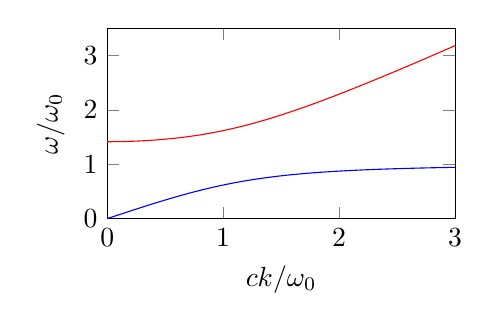
\begin{tikzpicture}\begin{axis}[width=6cm,height=4cm,xmin=0,xmax=3,ymin=0,ymax=3.5,xlabel={$ck/\omega_0$},ylabel={$\omega/\omega_0$}]
\addplot[blue,domain=0:3,samples=100]{sqrt((2+x*x-sqrt((2+x*x)^2-4*x*x))/2)};
\addplot[red,domain=0:3,samples=100]{sqrt((2+x*x+sqrt((2+x*x)^2-4*x*x))/2)};\end{axis}\end{tikzpicture}\quad
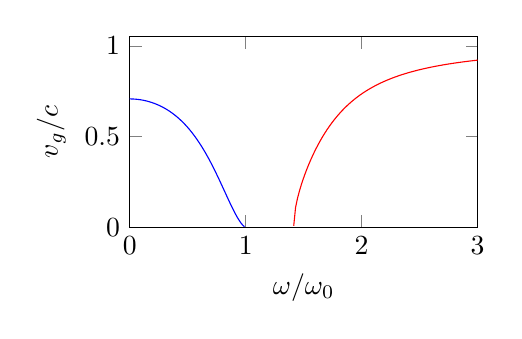
\begin{tikzpicture}\begin{axis}[width=6cm,height=4cm,xmin=0,xmax=3,ymin=0,ymax=1.05,xlabel={$\omega/\omega_0$},ylabel={$v_g/c$}]
\addplot[blue,domain=0:.99,samples=100]{1/(sqrt(1+1/(1-x*x))+x*x/(sqrt(1+1/(1-x*x))*(1-x*x)^2))};
\addplot[red,domain=1.4143:3,samples=100]{1/(sqrt(1+1/(1-x*x))+x*x/(sqrt(1+1/(1-x*x))*(1-x*x)^2))};\end{axis}\end{tikzpicture}\par
自绘无损$\omega_p=\omega_0$示意; 群速图不在禁带内连线.
\end{center}
\end{solution}
\originalsection{Kramers--Kronig和规则}
\begin{exercise}
原题6. 因果被动介电率趋$1-\omega_p^2/\omega^2$. (a) 导频谱和规则; (b) 证明正虚轴实值、单调趋1; (c) 证明上半平面无零点; (d) 对$1/\varepsilon_r$导关系与和规则.
\end{exercise}
\begin{solution}
真实响应满足$\varepsilon_r(-\omega^*)=\varepsilon_r(\omega)^*$; 原题省负号的表述需按此修正. 在因果解析、适当高频衰减的条件下, KK合并正负频率为
$\varepsilon_r(z)=1+(2/\pi)\int_0^\infty\omega'\operatorname{Im}\varepsilon_r(\omega')/(\omega'^2-z^2)\dd\omega'$, 上半平面成立, 实轴取主值.

(a) 大$z$展开$1/(\omega'^2-z^2)\sim-1/z^2$, 比较系数得$\omega_p^2=(2/\pi)\int_0^\infty\omega\operatorname{Im}\varepsilon_r\dd\omega$. 要求该矩收敛. (b) $z=i\xi$时分母$\omega'^2+\xi^2$为正, 结果实且$\partial_\xi\varepsilon_r(i\xi)=-(4\xi/\pi)\int\omega'\operatorname{Im}\varepsilon_r/(\omega'^2+\xi^2)^2\dd\omega'\le0$, 高频趋1.

(c) 令$y=\operatorname{Im}z>0$, 利用$z/(a^2-z^2)=[(a-z)^{-1}-(a+z)^{-1}]/2$, 得其虚部$y[|a-z|^{-2}+|a+z|^{-2}]/2>0$. 所以$\operatorname{Im}[z\varepsilon_r(z)]>0$, 不可能$\varepsilon_r(z)=0$. 实轴除零频外$\operatorname{Im}\varepsilon_r>0$也排除零点. 这里明确使用被动性, 仅解析性不足以得此结论.

(d) 既无上半平面零点, $\eta=1/\varepsilon_r$也解析, 高频$\eta=1+\omega_p^2/z^2+\cdots$. 同样KK给\[
\operatorname{Re}\eta(\omega)-1=\frac2\pi\PV\int_0^\infty\frac{\omega'\operatorname{Im}\eta(\omega')}{\omega'^2-\omega^2}\dd\omega'.
\]
和规则$-\omega_p^2=(2/\pi)\int_0^\infty\omega\operatorname{Im}(1/\varepsilon_r)\dd\omega$. 被动材料$\operatorname{Im}(1/\varepsilon_r)=-\operatorname{Im}\varepsilon_r/|\varepsilon_r|^2\le0$, 正负号自洽.
\end{solution}
